\section{Approaches to incorporate WordNet information}
Having the dataset of the previous section, we next try to improve our latest re-implementation Residual-Stacked Encoder\textsuperscript{$\dagger$} using WordNet. 
\subsection{Methods}
Unlike \ac{KIM}, which has shown an intuitive and successful strategy of incorporating WordNet into a neural network, the Residual-Stacked Encoder does not use inter-sentence attention. Without changing this, we therefore cannot likewise align words of $p$ with words of $h$ to identify their WordNet relation. We intend to leave the model with the plain sentence-encoding architecture, targeting the incorporation of external resources for general sentence representations thus by encoding each sentence individually \citep{nangia2017repeval}. Naturally, not being able to align words with each other poses a new difficulty, since the relations of WordNet are defined between two senses. Subsequentially, we apply other strategies, than directly encoding the relation of two words (or senses), explained below.
\subsubsection{Drawbacks of using insights of max-pooled sentence representations}
In Section §\ref{sec:understanding} we gained valid insights on the sentence representations and showed that these sucessfully can be used to change the meaning of sentence representations. Following these conclusions, a possible strategy is, to train the model in a way, that antonyms or co-hyponyms result in distinct high dimensions within the sentence representation, synonyms having the same high values and hypernyms a subset of hyponyms. Knowing reasonable values for each values within the dimensions, this could be broken down to a simple regression problem. Since we did not find an elegant way to naturally include this into the loss function, two possibilities exist:
\begin{itemize}
\item \textbf{Manually define the $\xi$ of dimensions:} The values for each word are defined before the training, w.r.t. the lexical relations that are shared amongst them, using automatic optimization techniques. The loss is defined w.r.t. those defined values for each word within a sentence.
\item \textbf{Regularily analyse the $\xi$ of dimensions:} Instead of defining the $\xi$ of each dimension beforehand, it can be gained by an anaylse step, similar to the one conducted for this work, every iteration. Knowing the dimensions, how they are already used by the model, they can slightly be adapted such that our wanted criteria is met. For instance, let the words $w_1$ and $w_2$ share a common close hypernym, thus both are co-hyponyms. After identifying the dimensions, that result in a high value coming from both words, some of tose dimensions are reserved for $w_1$ only, while others are reserved for $w_2$ only. This may also be achieved automatically, if dimensions are analysed for their high-valued words w.r.t. WordNet relations.
\end{itemize}
Both approaches severely lack the possibility of encoding words depending on their context into the sentence representation. While we gained some insights on the sentence-representations, it is insufficient to define them in a reasonable way. Even if this would be possible, it is not desired. Both strategies, especially the first, highly resemble traditional feature-engineering. Since the automatic feature selection is one of the key strengths of neural models \citep{bengio2013representation}, those strategies would rather be similar to a step backward than forward. Instead we identify to potential strategies, that are simpler to implement and would result in a broader applicability, not being tied to max-pooled sentence representations.

\subsubsection{Fuse WordNet information within the embedding-layer}
Additional information within the word-representations has the high advantage, of being very gerneral applicable. Following \cite{ruckle2018concatenated} we do not use exclusively retrained or adjusted word-embeddings. Instead, for each word $w$ we lookup the according word-vector within the original distributed GloVe embeddings and concatenate it with the corresponding word-vector of the same $w$ from the additional word-embeddings. If no corresponding vector for $w$ is present within those, we concatenate an zero-valued vector of the same dimensionality. Doing so, we do not chnge the original information of distributed word-embeddings such that the model may still rely on the same features, if they are useful. Even though some of the newly introduced might be redundant w.r.t. the orignal GloVe embeddings, some contain additional information, that the network can use to differentiate between words, that are highly similar in GloVe but mutually exclusive. Additional to doing this experiment with the mono-lingual attract-repel vectors, provided by \cite{ruckle2018concatenated}, we use two different word-vecor sources.

\paragraph*{Overfitting WordNet}
We apply a simple method to create addtitional word vectors $v$ that are similar for the words $w_1$ and $w_2$, if they are synonyms within WordNet, and different if $w_1$ and $w_2$ are antonyms or co-hyponyms. For this we extract samples ($w_1$, $w_2$, \texttt{relation}), whereas $w_1$ and $w_2$ are lemmas, that are linked via \texttt{relation} within WordNet, represented by their original GloVe embeddings. Using a two layer \ac{MLP}, we map each word-vector $w \in \mathbb{R}^{300}$ to $v \in \mathbb{R}^{20}$. In our last layer we apply tangens-hyperbolicus as non-linearity, to squeeze all values $v^i$ within $v$, with $v^i$ being the $i$th value within $v$, are in an appropriate range:  $ \forall i: [i \in \{x \in \mathbb{N} | x < 20\} \Rightarrow v^i \in \{x \in \mathbb{R} | -1 < x < 1\}]$. Let $w \in \mathbb{R}^{300 \times 1}$ be the original word-embedding, $W_1 \in \mathbb{R}^{100 \times 300}$ and $b_1 \in \mathbb{R}^{100 \times 1}$ the weight matrix and bias of the first layer, and $W_2 \in \mathbb{R}^{20 \times 100}$ and $b_2 \in \mathbb{R}^{20 \times 1}$ of the second layer respectively. The new word-vector $v$ is calculated as:
\begin{equation}
v = \tanh(W_2 \text{ reLU}(W_1w + b_1) + b_2)
\end{equation}
We optimize the representations $v_1$ and $v_2$, coming from ($w_1$, $w_2$, \texttt{relation}) using \ac{MSE} with the Eucledian Distance, which should be high, if the relation indicates, $w_1$ and $w_2$ are mutually exclusive, and low, if both are synonyms. Thus, we define $\theta=0$ for synonyms, and $\theta =10$, for antonyms and co-hyponyms (we bound the difference to $\frac{|v|}{2}$, with $|v|$ being the amount of dimensions of the new word-vectors, as it creates sufficiently distinct vectors):
\begin{equation}\label{eq:loss_embd}
\text{loss} = \frac{1}{2}\Bigg( \sqrt{\sum^{20}_{i=1}(v^i_1 - v^i_2)^2} - \theta\Bigg)^2
\end{equation}
We overfit on the lexical relations, extracted from WordNet, using the loss function in Equation (\ref{eq:loss_embd}), intending to memorize whether two words are compatible or not. This optimization process also updates the GloVe embeddings of $w$ during training.
\paragraph*{Adding categorical information}
Alternatively, especially targeting the detection of co-hyponyms, instead of concatenating different embeddings, we conctatenate each word $w$ with the distributed GloVe vector of the hypernyms of each $w$. The motivation is, that the network is able to identify, that two words share the same hypernym and hence, learning more subtle differences within the actual value-differences within both word-vectors. Due to WordNet's fine-grained ontology, we apply different strategies of taking the mean vector of one up to five hypernomys of a word. If hypernyms within WordNet consist of multi-word expressions, we take the word-embedding of the last word. For instance for ``single-reed instrument'', being the first hypernym of ``saxophone'', we concatenate the word-vector of ``saxophone'' with the word vector of ``instrument''.
\subsubsection{Fuse WordNet information within the sentence-representations}
It is very known, that neural networks do well in learning relevant features \citep{bengio2013representation}, however, as seen in Section §\ref{sec:additional_snli_set} and shown by \cite{gururangan2018annotation}, those features do not necessarily correspond with \ac{NLU}, but are heavily biased by dataset-specific patterns. These are not reduced, if we add additional informtion to the embeddings, thus we still need to rely on the full model to pick up on good features, yielding to correct decisions for the \textit{right} reason. \cite{gulccehre2016knowledge} show on a very different task, of detecting pentomino shapes, that deep neural networks may not even find the most useful features and can heavily leverage from human guidance when creating intermediate representations. In their very simple toy-scenario, this could be done by manually creating intermediate target representations, which is not easily possible for sentence-representations in \ac{NLP}. We thus continue training the nural network in an end-to-end manner. In order to guide the network in learning more useful sentence-representations, we create a second task, namely the helper-task, sharing some basic components with the maintask (predict the label for \ac{NLI}). Thus, both tasks rely on the same sentence representation, that will therefore encode relevant features for both tasks, whereas one can leverage from the features from the other. This is commonly known as multitask-learning and has shown to be successful to improve the generalization of shared representations \citep{nangia2017repeval}.
\paragraph*{Multitask architecture}
The multitask setup is visualized in Figure \ref{fig:mt_architecture}.
\begin{figure}[tph!]
\centering
	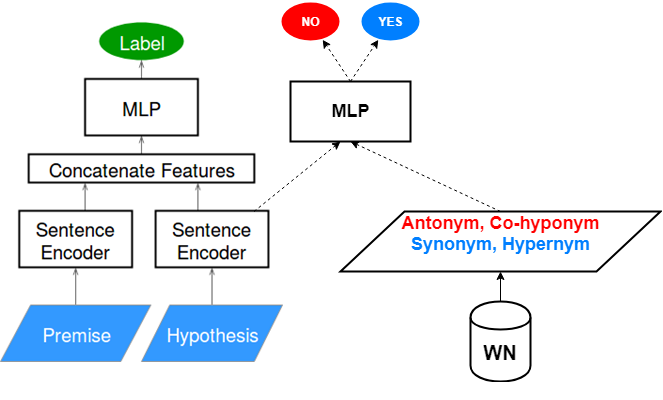
\includegraphics[totalheight=5.5cm]{fig/mt_architecture.png}
	\caption{Architecture of the Residual-Stacked Encoder with multitask learning for the sentence-representations.}
	\label{fig:mt_architecture}
\end{figure}
The left side shows the standard architecture of the Residual-Stacked Encoder, as defined in Section §\ref{sec:residual_encoder_def} Both sentences $p$ and $h$ are encoded using the same sentence encoder. The resulting sentence representations are concatenated with the additional features and classified by the final \ac{MLP} into on the three labels entailment, neutral or contradiction.The additonal \ac{MLP} on the right side is used for the helper task. We create the helper-task with the intention to force the model to encode differences between two words $w_1$ and $w_2$, if one is the antonym or co-hyponym of the other, into the sentence representations, as this essentially is used for the final prediction.  Likewise, if $w_1$ and $w_2$ are synonyms or $w_2$ is the hypernym of $w_1$ and thus entailed by it, we want this information to be encoded as well. In order to contain this information, which preumeably helps the generalization power of the main-task, within the sentence representation, we define our helper task, as a binary classification problem, whether a word is encoded within the sentence representation or not. For this, we consider both sentences $p$ and $h$ from a \ac{BoW} perspective. Let $S=\{w^0, w^1 , \ldots, w^{n-1}, w^n\}$ be the set of all $n$ distinct words $w$ within a sentence. We apply the same task for $p$ and $h$. Since we do not consider them simultaneously but individually, we define the helper-task using the general $S$ respectively for both. For each $w^i \in S$, we identify words from WordNet, being related to $w^i$ with one of the previously mentioned lexical semantic relations. Let $A$ be the set of words, who's meaning must be entailed by the sentence representation, thus $A$ contains all hypernyms and synonyms of all $w^i \in S$. Similarily, let $B$ be the set of words, who's meaning is \textit{not} entailed by the sentence, thus antonyms and co-hyponyms of all $w^i \in S$. Additionally, all $w^i$ that have related words via lexical semantic relations are also added to $A$. A sentence like ``People are watching a soccer game between Brazil and Mexico.'' may still cause conflicts, as $A$ contains ``Brazil'' and ``Mexico'', however they may also be present within $B$, being mutual co-hyponyms. To avoid conflicts, if several co-hyponyms are present within the same sentence, we ensure that $A$ and $B$ are not overlapping, by setting $B = B \setminus A$. The final helper-task takes a sentence representation $r$ and a word embedding $e$ as input, and must classify, whether $e$ belongs to $A$ or $B$, meaning whether $e$ is present (in the sense of entailment) within $r$ or not. Since the same embeddings are used and fine-tuned, this may also be seen similarily to further postprocess word vectors, like in Attract-Repel \citep{vulic2017specialising}, but additionally ensuring, those differences are propagated into the sentence representation. 

\paragraph*{Training}
The main-task and the helper-task are simultaneously trained. Thus, the combined loss, denoted as $loss_\text{combined}$, aggregating the loss for the main-task, denoted as $loss_\text{main}$, and for the helper task, denoted as $loss_\text{helper}$, as
\begin{equation}
\label{eq:multitask_aggregate}
\text{loss}_\text{combined} = \alpha \text{ loss}_\text{main} + (1 - \alpha)\text{ loss}_\text{helper}
\end{equation}
whereas $\alpha \in \{x \in \mathbb{R} | 0 \leq x \leq 1\}$ regulates the impact of the main-task, with a high value ($\alpha = 1$) only considering the main-task and a low value ($\alpha = 0$) only the helper-task. We train the network using a batchsize of 32. While $loss_\text{main}$ remains the original cross entropy, $loss_\text{helper}$ is also based on cross-entropy, yet is down-weighted for the following reason. Let $A_p$, $B_p$ and $A_h$, $B_h$ be $A$ and $B$ according to the definitions above for $p$ and $h$ respectively and $|A|$ denote the amount of samples within the set $A$. One can safely assume, that the amount of samples for the helper-task is tremendously higher than for the main task, as one single sample ($p$,$h$) here yields $|A_p|+|B_p|+|A_h|+|B_h| \gg 1$ samples in the helper-task. Let $b$ be the batch-size and $p^i$ and $h^i$ denote the $i$th $p$ or $h$ within a minibatch. We calculate $n$ to be the total amount of samples for the helper-task within the given batch:
\begin{equation}
n = \sum^b_{i=1}\Big(|A_{p^i}|+|B_{p^i}|+|A_{h^i}|+|B_{h^i}|\Big)
\end{equation}


reweight

For efficien

\paragraph*{Multitask variations}
We evaluate several implementations with small differences or changed hyperparameters, following the presented architecture. Those are described below, mostly differing in their impact on the sentence-representation. 
\begin{itemize}
\item \textbf{Size and amount of layers:} We evaluate different sizes of the helper-task \ac{MLP}. Naturally, the simpler the helper network (fewer layers and dimensions per layer), the more relevant information must be encoded within the representation. This should be preferrable, since finally we aim for the main-task to identify the same, hopefully meaningful, features, and we do not have further usage for the logic, implemented within the helper-task \ac{MLP}.
\item  \textbf{Dropout:} Similarily, by using dropout in the helper-task, we motivate the creation of redundant features within the sentence-representation.
\item \textbf{Reweighting tasks:} 
\end{itemize}
\subsection{Extraction of WordNet data}
\subsection{Integrating information into word-embeddings}
\subsubsection{Motivation}
\citep{rubinstein2015well} show something that distributional embeddings not always good (reread)
\subsubsection{Concatenating pre-trained word-embeddings}
\subsubsection{Concatenation categorical information}
\subsubsection{Analysis}
\subsection{Multitask Learning}
\citep{levy2015improving} show that embeddings not necessarily (reread)
\subsubsection{Motivation}
\subsubsection{Architecture}
\subsubsection{Approaches}
\paragraph{Different sizes of multitask MLP}
\paragraph{Introducing Dropout}
\paragraph{Introducing an additional shared layer}
\paragraph{Fixing multitasking network during training}
\paragraph{Focusing on original words within sentence representation}
\subsubsection{Analysis}
\subsubsection{Evaluation}

cite: An Overview of Multi-Task Learning
in Deep Neural Networks